\section{Eigenschaften von OPLs}
Dieser Abschnitt widmet sich den wichtigsten Eigenschaften von Operatorpräzedenzautomaten, wie die Äquivalenz zwischen OPG und OPA, der Äquivalenz von deterministischen und nichtdeterministischen OPAs und den Abschlusseigenschaften, sowie eine Einordnung von anderen Automatenklassen wie endliche Automaten und Visibly Pushdown Automaten. Weiterhin werden zu allen Eigenschaften die Beweise geführt.
\subsection{Äquivalenz von OPG und OPA}
Eine wesentliche Eigenschaft vieler Sprachklassen ist die Äquivalenz ihrer Grammatiken mit den Automaten. Mit dem vorgestellten OPA haben die OPL nun einen Automaten, der genau die Grammatik erkennt. Die Äquivalenz wird in beiden Richtungen gezeigt. \cite{precedence_automata, mso}

\subsubsection{Von OPGs zu OPAs}
\label{opgopa}
\begin{lemma}
Sei $G=(N,\Sigma, P, S)$ eine OPG. Dann kann ein OPA A konstruiert werden, sodass $L(G)=L(A)$. Weiterhin sei m die Summe der rechten Seite von Produktionsregeln in G. Dann hat A genau $O(m^2)$ Zustände.
\end{lemma}
\begin{proof}
Zunächst wird der nichtdeterministische OPA $A=(\Sigma, M, Q, I,F, \delta)$ aus einer gegebenen Grammatik mit derselben OPM konstruiert.
Ohne Beschränkung der Allgemeinheit wird angenommen, dass die Grammatik G keine leeren oder umbenennenden Regeln hat. Der OPA A wird nun so konstruiert, dass eine akzeptierende Berechnung dem Aufbauen eines Bottom-Up Ableitungsbaums in G gleicht. Der Automat führt eine Pushtransition aus, wenn das erste Terminal einer neuen rechten Regelseite gelesen wird. Eine Shift-transition  wird ausgeführt bei Terminalsymbolen innerhalb der rechten Seite einer Regel und schätzt nichtdeterministisch das Nichtterminal der linken Seite. Jeder Zustand enthält dabei zwei Informationen: Die erste Komponente repräsentiert dabei das Präfix der rechten Seite unter Konstruktion, während die zweite genutzt wird, um die rechte Seite, die vorher unter Konstruktion war, wiederherzustellen, wenn alle verschachtelten rechten Seiten fertiggestellt wurden.
Genau definiert wird die Konstruktion folgendermaßen: Sei 
\begin{center}
$\mathbb{P}={\alpha\in (N\cup\Sigma)^*\Sigma|\exists a\rightarrow\alpha\beta\in P}$
\end{center}
die Menge der Präfixe (die auf ein Terminalsymbol enden) der rechten Regelseiten in G. Weiter sei
\begin{center}
$\mathbb{Q}=\{\epsilon\}\cup\mathbb{P}\cup N$,\\
$Q=\mathbb{Q} \times (\{\epsilon\} \cup \mathbb{P})$, $I={(\epsilon, \epsilon)}$ und $F=S\times \{\epsilon\} \cup \{(\epsilon, \epsilon|\epsilon\in L(G)\}$
\end{center}

Anmerkung: $|\mathbb{Q}|=1+|\mathbb{P}|+|N|$ ist $O(m)$, also hat Q $O(m^2)$ Zustände\\
Die Transitionen sind folgendermaßen definiert für $a\in \Sigma, \quad \alpha, \alpha_1, \alpha_2\in\mathbb{Q}$ und $\beta, \beta_1, \beta_2 \in \mathbb{P} \cup \{\epsilon\}$:
\begin{itemize}
\item
$\delta_{push}\big ( (\alpha, \beta),a \big )\ni 
\begin{cases}
(a, \alpha) & if; \alpha \notin N, \\
(\alpha a, \beta) & if;  \alpha \in N, \\
\end{cases}$
\item
$\delta_{shift}\big ( (\alpha, \beta),a \big )\ni 
\begin{cases}
(\alpha a, \beta) & if; \alpha \notin N, \\
(\beta\alpha a, \beta) & if;  \alpha \in N, \\
\end{cases}$
\item
$\delta_{pop}\big ( (\alpha_1, \beta_1), (\alpha_2, \beta_2) \big ) \ni (A, \gamma)$, für jedes A, sodass\\
$\begin{cases}
A\rightarrow \alpha_1\in P & if; \alpha_1 \notin N,\\
A\rightarrow \beta_1\alpha_1 \in P & if; \alpha_1 \in N,\\
\end{cases}$ und $\gamma= 
\begin{cases}
\alpha_2 & if; \alpha_2 \notin N, \\
\beta_2 & if; \beta_2 \in N. \\
\end{cases}$
\end{itemize}
Die entstandenen Zustände von $\delta_{shift}$ und $\delta_{shift}$ sind eindeutig, während $\delta:{pop}$ mehrere Zustände produzieren könnte, abhängig von wiederholten rechten Regelseiten. Die Zustände, die von Push- und Shift-Transisitionen erreicht werden haben ihre erste Komponente in $\mathbb{P}$. Wenn der Zustand $(\alpha, \beta)$ nach einer Push-Transition erreicht wird, dann ist $\alpha$ das Präfix der rechten Regelseite, die gerade in Konstruktion ist und $\beta$ das Präfix, was vorher in Konstruktion war. In diesem Fall ist $\alpha$ entweder ein Terminalsymbol oder ein Nichtterminal, gefolgt von einem Terminal.

Wenn der Zustand $(\alpha, \beta)$ nach einer Shift-Transition erreicht wird, dann ist $\alpha$ die Konkatenation der ersten Komponente des vorherigen Zustands und dem gelesenen Terminal und $\beta$ ändert sich nicht vom vorigen Zustand.

Die Zustände, die von Pop-Transitionen erreicht werden, haben die erste Komponente in N: Wenn $(A, \gamma)$ so ein Zustand ist, dann ist A die linke Regelseite und $\gamma$ das Präfix, was vorher unter Konstruktion war.

Damit ist die Konstuktion des Automaten abgeschlossen. Die Äquivalenz zwischen G und A leitet sich nun aus den folgenden Lemmata ab.
\begin{lemma}
Sei x der Rumpf einer Kette und $\beta, \gamma \in \mathbb{P \cup \{ \epsilon\} }$. Dann gilt für alle $h \geq 1$: Aus $(\beta, \gamma) \stackrel{x}{\rightsquigarrow} q$ folgt die Existenz von $A\in N$, sodass $A\stackrel{*}{\Rightarrow}x$ in G und $q=(A, \beta)$
\end{lemma}
\begin{proof}
Beweis durch Induktion der Tiefe $h=d(x)$.
\paragraph*{Induktionsanfang: (h=1)}
Wenn h=1 ist, dann ist $x=a_1a_2...a_n$ der Rumpf einer einfachen Kette mit einer Stütze wie in \autoref{Support} (1) mit $q_0 = (\beta, \gamma)$ und $q_n+1=q$. Weiter folgt aus der Definition der Push- und Shift-Funktionen, dass $q_i=(a_1...a_i, \beta)$ für alle $1 \leq i \leq n$ und aufgrund der Definition der Popfunktion ($\beta \notin N$, aufgrund der Induktionssannahme) ist $q=(A, \beta)$, mit $A \rightarrow a_1...a_n=x$ in P. Die so konstruierte Stütze hat die Form 
\begin{center}
$(\beta, \gamma) \stackrel{a_1}{\rightarrow} (a_1, \beta) \dashrightarrow ... \dashrightarrow (a_1...a_{n-1}, \beta) \stackrel{a_n}{\dashrightarrow} (a_1...a_n, \beta) \stackrel{(\beta, \gamma)} {\Rightarrow} (A,\beta)$.
\end{center}
Somit ist $A\stackrel{*}{\Rightarrow}x$ in G und der Induktionsanfang ist abgeschlossen.
\paragraph{Induktionsschritt}
Für h>1 ist $x=x_0a_1x_1...a_nx_n$ der Rumpf einer zusammengesetzten Kette mit einer Stütze wie in \autoref{Support} (2) mit $q_0=(\beta, \gamma)$ und $q_{n+1}=q$. Weiterhin sei $q_i=(\beta, \gamma)$ für alle $0 \neq i \neq n$ (Genauer ist $\beta_0 = \beta$ und $\gamma_0 = \gamma$). Aus der Induktionssannahme folgt nun für jeden nichtleere Rumpf $x_i$ einer Kette mit einer geringeren Tiefe als h, existiert $X_i \in N$, sodass es $X_i \stackrel{*}{\Rightarrow} x_i$ in G gibt und $q_i=(X_i, \beta)$ ist. Somit kann die Stütze wie folgt konstruiert werden:
 \begin{eqnarray*}
(\beta, \gamma) \stackrel{x_0}{\rightsquigarrow} q_0^{\prime} \stackrel{a_1}{\rightarrow} (\beta_1, \gamma_1) \stackrel{x_1}{\rightsquigarrow} q_1^{\prime} \dashrightarrow ... \dashrightarrow q_{n-1} \stackrel{a_n}{\dashrightarrow} (\beta_n, \gamma_n) \stackrel{x_n}{\rightsquigarrow} q_n^{\prime} \stackrel {q_0^{\prime}} {\Rightarrow} q
\end{eqnarray*}\\
mit 
\begin{eqnarray*}
q_i^\prime = \begin{cases}
(\beta_i, \gamma_i) & if \; x_i = \epsilon \\
(X_i, \beta_i) & sonst
\end{cases}
\end{eqnarray*}
Nun wird aufgrund der Definition der Push- und Shift-Funktionen klar, dass für alle $i \neq 0,\; \beta_i = X_0a_1...X_{i-1}a_i$ gilt, egal ob $x_i$ leer ist oder nicht $(X_i=\epsilon$, wenn $x_i=\epsilon)$. Um jetzt den Zustand q, der mit der finalen Pop-Transition $\delta_{pop}(q_n^\prime, q_0^\prime)$ erreicht wird, zu berechnen, müssen vier verschiedene Fälle betrachtet werden (Sind $x_0, x_n$ leer oder nicht?), was genau in der Definition von $\delta_{pop}$ abgebildet ist. In allen Fällen hat q aber die Form $(A, \beta)$ mit $A \rightarrow X_0a_1X_1...X_na_nX_n$ in G.\\
 Somit ist der Beweis abgeschlossen.
\end{proof}

\begin{lemma}.
Sei x der Rumpf einer Kette und $A \in N$. Dann folgt aus $A \stackrel{*}{\Rightarrow} x$ in G, dass $(\beta, \gamma) \stackrel{x}{\rightsquigarrow}(A, \beta)$ für jedes $\beta, \gamma \in \mathbb{P} \cup \{\epsilon\}$.
\end{lemma}
\begin{proof}
Beweis durch Induktion auf die Tiefe h der Kette. 
\paragraph*{Induktionsanfang: (h=1)}
Wenn h=1 ist, dann ist x der Rumpf einer einfachen Kette und somit bedeutet $A \stackrel{*} {\Rightarrow} x$, dass $A \rightarrow x$ eine Produktion ist. Somit kann aufgrund der Definition von $\delta$ ($\beta \notin N$ aufgrund der Annahme) eine Stütze wie in \autoref{Support} (1) mit $q_0=(\beta, \gamma), \; q_{n+1}=q$ und $q_i=(a_1...a_i, \beta)$ für alle $i=1,2,...n$.
\paragraph*{Induktionsschritt:}
Wenn h > 1 ist, dann ist x der Rumpf einer zusammengesetzten Kette mit $x=x_0a_1x_1...a_nx_n$. Weiter folgt aus $A\stackrel{*}{\Rightarrow}x$ in G die Existenz von $X_0, X_1, ...,X_n \in \{\epsilon\}\cup N$ ($X_i = \epsilon, \; if \; x_i=\epsilon$), sodass $A\rightarrow X_0a_1X_1...a_nX_n$ und $X_i \stackrel{*}{\Rightarrow}x_i$. Der erste Schritt der Berechnung hängt davon ab, ob $x_0$ leer ist oder nicht. In beiden Fällen hat der Pfad jedoch die Form
\begin{eqnarray*}
(\beta, \gamma) \stackrel{x_0}{\rightsquigarrow} q_0^\prime \stackrel{a_1}{\rightarrow} (X_0a_1, \beta), \quad mit \quad q_0^\prime= = \begin{cases}
(\beta, \gamma) & if \; x_0 = \epsilon \\
(X_0, \beta) & sonst \\
\end{cases}
\end{eqnarray*}
Die Berechnung hängt auch weiter davon ab, ob $x_1, x_2,...x_{n-1}$ leer ist oder nicht sind. Jedoch gilt aufgrund der Induktionsannahme und der Definition von $\delta_{shift}$, dass der Automat nach dem Lesen von $a_i$ den Zustand $(X_0a_1...X_{i-1}a_i, \beta)$ für jedes $i=1,...,n$ erreicht mit dem Pfad 
\begin{multline*}
(\beta, \gamma) \stackrel{x_0}{\rightsquigarrow} q_0^\prime \stackrel{a_1}{\rightarrow} (X_0a_1, \beta) \stackrel{x_1}{\rightsquigarrow}q_1 \stackrel{a_2}{\dashrightarrow}(X_0a_1X_1a_2, \beta) \stackrel{x_2}{\rightsquigarrow} q_2^\prime \stackrel{a_3}{\dashrightarrow}... \\
...\stackrel{a_n}{\dashrightarrow} (X_0a_1...X_{n-1}a_n, \beta)
\end{multline*}
Wenn $x_n \neq \epsilon$ geht die Berechnung weiter mit dem letzten Schritt
\begin{eqnarray*}
(X_0a_1...X_{n-1}a_n, \beta) \stackrel{x_n}{\rightsquigarrow} (X_n, X_0a_1...X_{n-1}a_n).
\end{eqnarray*}
Damit endet die Berechnung nun mit einer Pop-Transition. Die vier Fälle, die durch leere $x_0, x_n$ entstehen, sind durch die Defintion von $\delta_{pop}$ abgedeckt. In allen Fällen wurde aber eine Stütze, die auf den Zustand $(A, \beta)$ endet, konstruiert und der Beweis ist abgeschlossen.
\end{proof}
Somit wurde in beide Richtungen gezeigt, dass die Konstruktion des Automaten genau die Ketten der Grammatik repräsentiert und es für jede Stütze eine Ableitung in G gibt. Damit ist der Beweis abgeschlossen 
\end{proof}


\subsubsection{Von OPAs zu OPGs}
Die Konstruktion einer äquivalenten Grammatik G aus einem OPA A ist deutlich einfacher als andersrum, was aus der Struktur, die durch OPMs vorgegeben ist, resultiert.
\begin{lemma}
Für einen OPA A kann eine äquivalente Grammatik G konstruiert werden, sodass L(G)=L(A) gilt.
\end{lemma}
\begin{proof}
Die Konstruktion setzt das Prinzip der Stützen direkt und intuitiv in die Grammatik um.
Für einen gegebenen Automaten $A=(\Sigma, M, Q, I, F, \delta)$ wird nun die Grammatik $G=(\Sigma, N, P, S)$ konstruiert:
\begin{itemize}
\item Die Nichtterminale N sind 4-Tupel $(a,q,p,b)\in \Sigma \times Q \times Q \times \Sigma$ und werden als $(^bp,q^b)$ beschrieben. \\
Die Regeln in P werden wie folgt konstruiert:
\item
Für jeden Support \autoref{Support}(1) einer einfachen Kette wird die Regel 
\begin{equation}
(^{a_0} q_0, q_{n+1} \phantom{}^{a_{n+1}})\rightarrow a_1a_2...a_n
\end{equation}
hinzugefügt. Wenn $a_0=a_{n+1}=\#, \; q_0 \in I$ und $q_{n+1} \in F$, dann ist $(^\#q_0,q_{n+1}^\#)$ in S.
\item
Für jeden Support \autoref{Support}(2) einer zusammengesetzten Kette wird die Regel 
\begin{equation}
(^{a_0}q_0, q_{n+1} \phantom{}^{a_{n+1}})\rightarrow \Delta_0a_1\Delta_1a_2...a_n\Delta_n
\end{equation}
hinzugefügt, wobei für alle $0 \leq i \leq n, \quad \Delta_i = (^a_i q_i, q_i^{\prime a_{i+1}})$, wenn $x_i$ der Kette nicht leer ist, sonst $\Delta_i = \epsilon$. Wenn $a_0=a_{n+1}=\#, \; q_0 \in I$ und $q_{n+1} \in F$, dann ist $(^\#q_0,q_{n+1}^\#)$ in S.
\item
Wenn der Automat $\epsilon$ akzeptiert, wird eine Regel $S\rightarrow \epsilon$ hinzugefügt. S darf nicht in anderen Regeln verwendet werden.
\end{itemize}
Durch die Definition der Zustände ist $|N|$ maximal $O(|\Sigma|^2 * |Q|^2)$.
Für die Konstruktion wurden die Stützen direkt in Regeln übersetzt. Die Äquivalenz sollte daher trivial sein.


\end{proof}

\subsection{Deterministischer vs. Nichtdeterminstischer OPA}
Die vorherige Definition von OPAs war nichtdeterministisch. Eine vorteilhafte Eigenschaft von OPAs ist nun die Äquivalenz der deterministischen und nichtdeterministischen Version. Dadurch unterscheidet sich diese Familie der Automaten wesentlich von den Kellerautomaten. \\
In diesem Abschnitt geht es um die Definition und die Konstruktion eines solchen deterministischen OPAs und um die Lemmata, die nötig sind, um die Korrektheit zu beweisen. \cite{precedence_automata}
\begin{definition}[Deterministischer OPA]
Ein OPA $A=(\Sigma, M, Q, I, F, \delta)$ ist deterministisch, wenn gilt:
\begin{itemize}
\item
I besteht aus nur einem Element 
\item
$\delta: Q \times \{Q \cup \Sigma\} \rightarrow Q\}$ \\
($\delta$ bildet auf Q ab, anstatt auf $\mathcal{P}(Q)$)
\end{itemize}
\end{definition}
Anmerkung: Bei dem Startzustand wird nicht zwischen dem einzelnen Element und einer Singleton-Menge unterschieden.\\
Bei der Konstruktion eines deterministischen OPA aus einem nichtdeterministischen wird folgende Grundidee verwendet: Es muss sichergestellt werden, dass die Pop-Moves von verschiedenen Läufen des nichtdeterministischen Automaten nicht mit falschen initialen und finalen Zuständen vermischt werden. Dazu werden Informationen zu dem Pfad, die der Automat seit dem Push-Move, also dem Beginn einer Kette, genommen hat, gesammelt. Weiterhin wird jeder Zustand des deterministischen Automaten als Menge von Zustandspaaren defininiert. Der deterministische Automat simuliert den nichtdeterministischen Lauf mithilfe des ersten Zustand des Paares und speichert den Zustand, von dem aus der Push-Move ausging, im zweiten Zustand. Die deterministischen Pop-Moves werden anhand  der nichtdeterministischen Pop-Moves die für den ersten Zustand und dem Zustand, der vor dem letzten Push-Move erreicht wurde (was dem obersten Stackeintrag entspricht), definiert sind simuliert.\\
Das wird nun in einem Lemma formal ausgedrückt und bewiesen.
\begin{lemma}
\label{lemma_Deter}
Aus einem nichtdeterminischen OPA A mit s Zuständen kann ein äquivalenter deterministischer OPA $\tilde{A}$ mit $2^{O(s^2)}$ Zuständen konstruiert werden.
\end{lemma}
\begin{proof}
Sei $A=(\Sigma, M, Q, I, F, \delta)$ ein nichtdeterministischer OPA. Der deterministsiche OPA $\tilde{A}=(\Sigma, M, \tilde{Q}, \tilde{I}, \tilde{F}, \tilde{\delta}$ wird wie folgt definiert:
\begin{itemize}
\item
$\tilde{Q} = \mathcal{P}(Q \times (Q \cup \{\top\}))$, wobei $\top \notin Q$ für die Basis der Berechnungen (leerer Stack) steht. Zustände in $\tilde{Q}$ werden mit K bezeichnet
\item
$\tilde{I}=I\times \{\top \}$ ist der Startzustand
\item
$\tilde{F}=\left\{K|K \cap (F \times \{\top\}) \neq \emptyset\right\}$
\item
$\tilde{\delta}: \tilde{Q} \times (\Sigma \cup \tilde{Q})\rightarrow \tilde{Q}$ ist die Übergangsfunktion, definiert als Vereinigung aus den drei Teilfunktionen:\\[2ex]
$\tilde{\delta}_{push}: \tilde{Q} \times \Sigma \rightarrow \tilde{Q}$ ist definiert als: 
\begin{equation*}
\tilde{\delta}_{push}(K, a) = \bigcup\limits_{(q,p) \in K} \{(h,q)|h \in \delta_{push}(q,a)\}
\end{equation*}
$\tilde{\delta}_{shift}: \tilde{Q} \times \Sigma \rightarrow \tilde{Q}$ ist definiert als: 
\begin{equation*}
\tilde{\delta}_{shift}(K, a) = \bigcup\limits_{(q,p) \in K} \{(h,p)|h \in \delta_{shift}(q,a)\}
\end{equation*}
$\tilde{\delta}_{pop}: \tilde{Q} \times \tilde{Q}\rightarrow \tilde{Q}$ ist definiert als: 
\begin{equation*}
\tilde{\delta}_{pop}(K_1, K_2) = \bigcup\limits_{(r,q) \in K_1, (q,p)\in K_2} \{(h,p)|h \in \delta_{pop}(r,q)\}
\end{equation*}
\end{itemize}
Die Zahl s der Zustände wächst exponential: Sei s = $|Q|$ die Anzahl der Zustände vom nichtdeterministischen Automaten A, dann ist $|\tilde{Q}| = 2^{|Q| * |Q \cup \{\top\}|}$. Also hat $\tilde{A}$  $2^{O(s^2)}$ Zustände.\\
Die Äquivalenz der beiden Automaten basiert auf den Aussagen der beiden folgenden Lemmata, die in die jeweilige Richtung zeigen, dass äquivalente Supports gebildet werden:
\begin{lemma}
Sei y der Rumpf einer Kette mit der Stütze $q\stackrel{y}{\rightsquigarrow} q^\prime$ in A. Dann gilt für alle $p \in Q$ und $K \in \tilde{Q}$, wenn $(q,p) \in K$, dann existiert eine Stütze $K\stackrel{y}{\rightsquigarrow} K^\prime$ mit $(q^\prime, p) \in K^\prime $
\end{lemma}
\begin{proof}
\label{lemma_deter1}
Beweis durch Induktion der Tiefe h = $d(y)$. 
\paragraph{Induktionsanfang: (h = 1)}\ \\
Wenn h = 1 ist, dann ist $y = a_1a_2...a_n$ und die Stütze in A hat die Form $q  \stackrel{a_1}{\rightarrow} q_1 \dashrightarrow ... \dashrightarrow q_{n-1} \stackrel{a_n}{\dashrightarrow} q_n \stackrel {q_0} {\Rightarrow} q^\prime$.\\[1,5ex] Sei \\[1ex]
\begin{tabular}[c]{l}
$K_1=\tilde{\delta}_{push}(K, a_1)$,\\
$K_i=\tilde{\delta}_{shift}(K_{i-1}, a_1)\quad$, für jedes $i=2,...,n$\\
$K^\prime = \tilde{\delta}_{pop}(K_n, K)$.
\end{tabular}
\\[1,5ex]Dann ist
\begin{equation*}
K\stackrel{a_1}{\rightarrow} K_1 \stackrel{a_2}{\dashrightarrow} ... \stackrel{a_{n-1}}{\dashrightarrow} K_{n-1} \stackrel{a_n}{\dashrightarrow} K_n \stackrel {q_0} {\Rightarrow} K^\prime. 
\end{equation*}
die Stütze in $\tilde{A}$. Weiterhin gilt für $(q,p) \in K$ aufgrund der Definition von $\tilde{\delta}$:\\
\begin{tabular}{l l}
$(q_1,q) \in K_1$, & da $q_1 \in \delta_{push}(q, a_1)$, \\
$(q_i, q) \in K_i$, & da $q_i \in \delta_{shift}(q_{i-1})$, \\
$(q^\prime, p) \in K^\prime$, & da $q^\prime \in \delta_{pop}(q_n, q)$ 
\end{tabular}
\paragraph{Induktionsschritt}\ \\
Nun gelte Induktionsannahme für Stützen mit einer geringeren Tiefe als h. Weiter sei $y = x_0a_1x_1a_2...a_nx_n$ mit der Tiefe h und der Stütze $q \stackrel{x_0}{\rightsquigarrow} q_0^{\prime} \stackrel{a_1}{\rightarrow} q_1\stackrel{x_1}{\rightsquigarrow} q_1^{\prime} \dashrightarrow ... \dashrightarrow q_{n-1} \stackrel{a_n}{\dashrightarrow} q_n \stackrel{x_n}{\rightsquigarrow} q_n^{\prime} \stackrel {q_0^{\prime}} {\Rightarrow} q^\prime$, wobei $q_i^\prime = q_i$, wenn $x_i = \epsilon$ und jedes nichtleere $x_i$  eine geringere Tiefe als h hat. Dann kann aufgrund der Induktionsannahme und der Definition von $\tilde{\delta}$ eine Stütze
\begin{eqnarray*}
K \stackrel{x_0}{\rightsquigarrow} K_0^{\prime} \stackrel{a_1}{\rightarrow} K_1\stackrel{x_1}{\rightsquigarrow} K_1^{\prime} \dashrightarrow ... \dashrightarrow K_{n-1} \stackrel{a_n}{\dashrightarrow} K_n \stackrel{x_n}{\rightsquigarrow} K_n^{\prime} \stackrel {K_0^{\prime}} {\Rightarrow} K^\prime 
\end{eqnarray*}
konstruiert werden und weil $(q,p) \in K$ ist, gilt:\\[1ex]
\begin{tabular}[c] {l l}
$(q_0^\prime, p) \in K_0^\prime $  & durch die Induktionsannahme auf die Stütze $q \stackrel{x_0}{\rightsquigarrow} q_0^\prime$ \\
$ (q_1, q_0^\prime) \in K_1$, & denn $q_1 \in \delta_{push}(q_0^\prime, a_1)$ \\
$(q_1^\prime, q_0^\prime) \in K_1^\prime$, & durch die Induktionsannahme auf die Stütze $q_1 \stackrel{x_1}{\rightsquigarrow} q_1^\prime$\\ 
$ (q_i, q_0^\prime) \in K_i$, & denn $q_i \in \delta_{shift}(q_{i-1}^\prime, a_1)$ für jedes $i=2,...,n$ \\
$(q_i^\prime, q_0^\prime) \in K_i^\prime$, & durch die Induktionsannahme auf die Stütze $q_i \stackrel{x_i}{\rightsquigarrow} q_i^\prime$\\ 
$ (q^\prime, p) \in K^\prime$, & denn $q^\prime \in \delta_{pop}(q_n, q_0^\prime)$ \\
\end{tabular}
Und dadurch ist der Beweis abgeschlossen.
\end{proof}
Die Aussage des nächsten Lemmas führt genau anders herum, vom Automaten $\tilde{A}$ zu A.
\begin{lemma}
\label{lemma_deter2}
Sei y der Rumpf einer Kette mit der Stütze $K \stackrel{y}{\rightsquigarrow} K^\prime$ in $\tilde{A}$. Dann gilt für alle $p, q^\prime \in Q$: Wenn $(q^\prime, p) \in K^\prime$, dann existiert eine Stütze $q \stackrel{y}{\rightsquigarrow} q^\prime$ in A.
\end{lemma}
\begin{proof}
Zunächst ein paar Anmerkungen, die für den Beweis verwendet werden:
\renewcommand{\labelenumi}{\roman{enumi})}
\begin{enumerate}
\item
Aus der Definition von $\delta_{push}$ folgt: Wenn es $\bar{K} \stackrel{a}{\rightarrow} K$ in $\tilde{A}$ gibt mit $(\bar{q}, q) \in K, \quad (q,p) \in \bar{K}$, dann gibt es $q \stackrel{a}{\rightarrow} \bar{q}$ in A.
\label{rem1}
\item
Aus der Definition von $\delta_{shift}$ folgt: Wenn es $\bar{K} \stackrel{a}{\dashrightarrow} K$ in $\tilde{A}$ gibt mit $(r,q) \in K$, dann existiert ein $\bar{q} \in Q$, sodass $\bar{q} \stackrel{a}{\dashrightarrow} r$ in A und $(\bar{q}, q) \in K$.
\label{rem2}
\item
Aus der Definition von $\delta_{pop}$ folgt: Wenn es $\bar{K} \stackrel{K}{\Rightarrow} K$ in $\tilde{A}$ gibt mit $(q^\prime q) \in \bar{K}$, dann existiert ein Paar $(r,q) \in \bar{K}$, sodass $(q,p)\in K$ und es gibt $r \stackrel{q}{\Rightarrow} q^\prime$ in A.
\label{rem3}
\end{enumerate}

Beweis durch Induktion auf die Höhe $h=d(y)$ 
\paragraph*{Induktionsanfang: (h=1)}
Wenn h=1 ist, dann ist $y=a_1a_2...a_n$ mit der Stütze $K\stackrel{a_1}{\rightarrow} K_1 \stackrel{a_2}{\dashrightarrow} ... \stackrel{a_{n-1}}{\dashrightarrow} K_{n-1} \stackrel{a_n}{\dashrightarrow} K_n \stackrel {q_0} {\Rightarrow} K^\prime.$ Sei $(q^\prime, p) \in K$, dann gibt es wie in Anmerkung \ref{rem3} in $\tilde{A}$ ein Paar $(q_n, q) \in K$, sodass $(q,p) \in K$ und $q_n \stackrel{q}{\Rightarrow} q^\prime$. Weiterhin folgt aus Anmerkung \ref{rem2} mit $(q_n, q) \in K$ und  $K_{n-1} \stackrel{a_n}{\dashrightarrow} K_n$ die Existenz eines Zustandes $q_{n-1} \in Q$, sodass $(q_n,q) \in K_{n-1}$ und $q_{n-1} \stackrel{a_n}{\dashrightarrow} q_n$. Auf gleiche Weise gilt für alle $i=n-2,...,1$, dass es $q_i \in Q$ gibt, sodass $(q_i,q) \in K_i$ und $q_i \stackrel{a_{i+1}}{\dashrightarrow} q_{i+1}$ Schließlich folgt aufgrund Anmerkung \ref{rem1} aus $K\stackrel{a_1}{\rightarrow} K_1$, $(q_1, q) \in K_1$ und $(q, p) \in K$, dass es $q \stackrel{a_1}{\rightarrow} q_1$ in A gibt. So wurde gezeigt, dass es eine Stütze für y gibt.
\paragraph*{Induktionsschritt} 
Nun gelte die Induktionsannahme für eine geringere Tiefe als h. Weiter sei $y=x_0a_1x_1a_2...a_nx_n$ mit der Tiefe h und der Stütze $K \stackrel{x_0}{\rightsquigarrow} K_0^{\prime} \stackrel{a_1}{\rightarrow} K_1\stackrel{x_1}{\rightsquigarrow} K_1^{\prime} \dashrightarrow ... \dashrightarrow K_{n-1} \stackrel{a_n}{\dashrightarrow} K_n \stackrel{x_n}{\rightsquigarrow} K_n^\prime \stackrel{K_0^{\prime}} {\Rightarrow} K^\prime$, wobei $K_i^\prime = K_i$, wenn $x_i= \epsilon$ und jedes nichtleere $x_i$ hat eine geringere Tiefe als h. Sei $(q^\prime, p) \in K^\prime$. Da es aufgrund von Anmerkung \ref{rem3} $K_n^\prime \stackrel{K_0^\prime} {\Rightarrow} K^\prime$ gibt, existiert ein Paar $(q_n^\prime, q_0^\prime) \in K_n^\prime$ in $\tilde{A}$ mit $(q_0^\prime, p) \in K_0^\prime$ und $q_n^\prime \stackrel{q_0^\prime}{\Rightarrow} q^\prime$. Wenn $x_n \neq \epsilon$ existiert aufgrund der Induktionsannahme, da $(q_n^\prime, q_0^\prime) \in K_n^\prime$, eine Stütze $q_n \stackrel{x_n}{\rightsquigarrow} q_n^\prime$ mit $(q_n, q_0^\prime \in K_n$. Auf gleiche Weise gilt für alle $i=n-1,...2,1$: Es existieren $q_i^\prime$ und $q_i$ ($q_i^\prime=q_i$, wenn $x_i= \epsilon$), sodass es $q_i \stackrel{x_i}{\rightsquigarrow} q_i^\prime \stackrel{a_{i+1}}{\dashrightarrow}q_{i+1}$ in A gibt,

\begin{tabular}{l p{8cm}}
mit $(q_i^\prime, q_0^\prime) \in K_i^\prime$ & (Aufgrund von Anmerkung \ref{rem2}, da $K_i^\prime \stackrel{a_{i+1}}{\dashrightarrow} K_{i+1}$ in $\tilde{A}$ und $(q_{i+1}, q_0^\prime) \in K_{i+1}$)\\

 und $(q_i^\prime, q_0^\prime) \in K_i$ & (Aufgrund der Induktionsannahme, da $K_i \stackrel{x_i}{\rightsquigarrow} K_i^\prime$ in $\tilde{A}$ und $(q_i^\prime, q_0^\prime) \in K_i^\prime$).
  \end{tabular}\\
 Das gilt speziell auch für $q_1 \stackrel{x_1}{\rightsquigarrow}q_1^\prime$ mit $(q_1, q_0^\prime) \in K_1$. Weiterhin gibt es $(q_0^\prime \stackrel{a_1}{\rightarrow} q_1$, da $K_0^\prime \stackrel{a_1} {\rightarrow} K_1$ und $(q_0^\prime, p) \in K_0^\prime$ (Anmerkung \ref{rem1}).
 
 Schließlich folgt aus der Induktionsannahme, da $(q_0^\prime, p) \in K_0^\prime$ und $K\stackrel{x_0}{\rightsquigarrow} K_0^\prime$, wenn $x_0 \neq \epsilon$ existiert ein Zustand $q \in Q$, sodass $q \stackrel{x_0}{\rightsquigarrow} q_0^\prime$ in $\tilde{A}$ mit $(q,p) \in K$. Somit haben wir eine Stütze nach \autoref{Support} (2) konstruiert und der Beweis ist abgeschlossen.
  \end{proof}
Um den Beweis von \autoref{lemma_Deter} zu vervollständigen muss noch bewiesen werden, dass eine akzeptierende Berechnung für y in A gibt, dies auch in $\tilde{A}$ zutrifft. 

Sei $y \in L(A)$. Dann gibt es eine Stütze $q \stackrel{y} {\rightsquigarrow} q^\prime$, wobei $q\in I, q^\prime \in F$. Dann folgt aus \autoref{lemma_deter1} für $(q_0, \top) \in K=I \times \{\top\}$, dass eine Stütze $K \stackrel{y}{\rightsquigarrow}K^\prime$ in $\tilde{A}$ mit $(q^\prime, \top) \in K^\prime $. $q^\prime \in F$ impliziert $K^\prime \in F^\prime$.
Andersherum sei $y \in L(\tilde{A})$. Dann hat y eine Stütze $\tilde{K}\stackrel{y}{\rightsquigarrow}K^\prime$ in $\tilde{A}$ mit $K^\prime \in \tilde{F}$. D.h., es existiert ein $q^\prime \in F$, sodass $(q^\prime, \top) \in K^\prime$. Aufgrund von \autoref{lemma_deter2} gibt es eine Stütze $q \stackrel{y} {\rightsquigarrow} q^\prime$ in A mit $(q^\prime, \top) \in \tilde{K}$ und daraus folgt $q \in I$. Somit definiert $q\stackrel{y}{\rightsquigarrow}q^\prime$ eine akzeptierende Berechnung für y in A.
Damit ist der Beweis abgeschlossen. 
\end{proof}

An dieser Stelle folgt eine weitere interessante Eigenschaft in Bezug auf Determinismus der Automaten, die  durch die Konstruktion aus einer Grammatik wie in \ref{opgopa} entstehen.
\begin{corollary}
Wenn die Ausgangsgrammatik in Fischer Normalform ist, dann ist der konstruierte Automat deterministisch.
\end{corollary}
Diese Behauptung folgt direkt aus der Konstruktion, in der die Werte, die durch $\delta_{push}$ und $\delta_{shift}$ definiert sind, immer Singletons sind und die $\delta_{pop}$-Funktion produziert soviele Zustände, wie es linke Regelseiten mit denselben rechten Regelseiten gibt. Eben diese letzte Eigenschaft wird in Fischernormalform verhindert, da es keine sich wiederholenden rechten Regelseite gibt. Also ist der resultierende Automat deterministisch. 

\subsection{Abgeschlossenheit}
OPG weisen wie reguläre Sprachen und im Gegensatz zu deterministisch-kontextfreien Sprachen Abgeschlossenheit unter typischen Sprachoperationen auf: Vereinigung, Komplement, Schnitt, Spiegelung, Präfix, Suffix, Konkatenation und Kleene-*.
Diese Eigenschaften werden auf Ebene der Grammatiken betrachtet. In \cite{algebraic_properties} formulieren Reghizzi und Mandrioli ein algebraisches Gitter und umfangreiche algebraische Eigenschaften, unter anderem eine partielle Ordnung und folgern daraus die Abgeschlossenheit unter Vereinigung, Schnitt und Komplement. Zuvor müssen zunächst allerdings noch ein paar Definitionen getätigt werden. 

\begin{definition}[Homogene Normalform]
Eine OPG ist in homogener Normalform, wenn sie in Fischer Normalform ist und für alle Regeln $A\rightarrow \alpha$, außer $A=S$ gilt $\mathcal{L}(A) = \mathcal{L}(\alpha) \; \wedge \; \mathcal{R}(A) = \mathcal{R}(\alpha)$.
Sei $\mathcal{H}$ die Klasse der homogenen OPGs.
\end{definition}
Das bedeutet, dass in einer homogenen Grammatik alle Regeln eines Nichtterminals die gleichen Terminalsets haben. Für jede OPG G kann eine strukturell äquivalente OPG H effektiv konstruiert werden. Die nächsten Definitionen betreffen die rechts-begrenzten Operatorpräzedenzgrammatiken.
\begin{definition}[freie OPG und Max-Grammatik]\ \\
\begin{itemize}
\item
Eine OPG G ist frei, wenn sie in homogener Normalform ist und für alle Nichtterminale A,B $\neq$ S gilt $\mathcal{L}_G(A) = \mathcal{L}_G(B) \wedge \mathcal{R}_G(A)=\mathcal{R}_G(B)$ impliziert $A=B$.
\item
 Für eine OPM M ist $\mathcal{F}(M)=\{F|F \; ist \; frei \; \wedge \; OPM(F) \subseteq M\}$ die Klasse der freien präzedenzkompatiblen OPGs.
 \item
 Für eine OPM M und $k \geq 1$, existiert eine eindeutige freie OPG $G_{M,k}$ mit $OPM(G_{M,k})= M \wedge \forall G \in C_{M,k}: L(G) \subseteq L(G_{M,k})$ \\
 Eine solche Grammatik $G_{M,k}$ wird als Max-Grammatik bezeichnet.
\end{itemize}
\end{definition}
Die Teilmengen Relation zwischen den Regelmengen der Grammatiken $F_1, F_2 \in \mathcal{F}(M)$ induziert eine partielle Ordnung $F_1 \leq F_2$ der freien Grammatiken. In \cite{algebraic_properties} wird ein algebraisches Gitter definiert mit dieser partiellen Ordnung, sodass die Max-Grammatik das oberste Element ist.

\begin{definition}
Sei $H=(N, \Sigma, P, S)$ eine homogene OPG mit OPM M. Die Mappingfunktion 
\begin{align*}
W: N \setminus \{S\} \rightarrow \mathcal{P}(\Sigma) \times \mathcal{P}(\Sigma)
\end{align*}
ist definiert als
\begin{align*}
W(A)=\left(\mathcal{L}(A), \mathcal{R}(A)\right)
\end{align*}
und wird intuitiv für die Regeln erweitert ($W(a)=a, \forall a\in \Sigma$). Eine freie Grammatik $F=W(H)$ ist dann $F=(W(N) \cup \{S\}, \Sigma, W(P), S)$.
\end{definition}

\begin{lemma}
\label{lemma54}
Aus $\L(\tilde{H}) \subseteq L(\tilde{F})$ mit $H \in \mathcal{H}, F \in \mathcal{F}$ folgt $W(H) \leq F.$
\end{lemma}
Durch die Mappingfunktion W wird $\mathcal{H}$ in disjunkte Klassen aufgeteilt. Für jede dieser Klassen $W^{-1}(F)$gilt:  $\forall H \in W^{-1}(F)$ mit $F\in \mathcal{F}$ gilt: $L(H) \subseteq L(F)$.

 Die Klasse der freien OPGs, die einer freien OPG F in der partiellen Ordnung vorangehen wird als $\mathcal{F}(F)=\{F^\prime \in \mathcal{F} | F^\prime \leq F\}$ definiert. Weiterhin wird die Klasse der homogenen OPGs für eine freie Grammatik definiert: $\mathcal{H}(F)=\{H \in \mathcal{H}|W(H)\in \mathcal{F}(F)\}$. Praktisch bedeutet das $\mathcal{H}(F)$ enthält alle homogenen Grammatiken, deren Regel die gleiche Form haben wie F. Daraus folgt, dass die OPMs dieser Grammatiken mit der OPM(F) kompatibel sind.

\begin{theorem}[Vereinigung]
Die Menge der Sprachen $\{L(H)|H \in \mathcal{H}(F)\}$ ist abgeschlossen unter Vereinigung
\end{theorem}
\begin{proof}
Sei $H_1=(N_1, \Sigma, P_1, S) \in W^{-1}(F_1)$ und $H_2=(N_2, \Sigma, P_2, S) \in W^{-1}(F_2)$ mit $F_1, F_2 \in \mathcal{F}(F)$. O.b.d.A. wird angenommen, dass $V_1 \cap V_2 = \{S\}$. Es wird nun die vereinigte Grammatik $G=(N_1 \cup N_2, \Sigma, P_1 \cup P_2, S)$ konstruiert und es gilt $L(G)=L(H_1) \cup L(H_2)$. Aus $OPM(H_1), OPM(H_2) \leq OPM(F)$ und den Definitonen der algebraischen Eigenschaften wird $L(\tilde{H_1}) \cup L(\tilde{H_2}) \subseteq L(\tilde{F_1}) \cup L(\tilde{F_2}) \subseteq L(\widetilde{F_1 \cup F_2}) \subseteq \tilde{F^\prime}$ gefolgert. Jetzt wird aus G eine homogene OPG H konstruiert, sodass $L(\tilde{G})=L(\tilde{H}$. Da $L(\tilde{H}) \subseteq L(\tilde{F})$ folgt aus \ref{lemma54}, dass $W(H) \leq F$ und damit ist der Beweis abgeschlossen. 
\end{proof}


\begin{theorem}[Komplement]
Die Menge der Sprachen $\{L(H)|H \in \mathcal{H}(F)\}$ ist abgeschlossen unter Komplement zu $L(F)$.
\end{theorem}
\begin{proof}
Sei $H \in \mathcal{H}(F)$, dann ist $L(H) \subseteq L(F)$. Es folgt aus der Definition der algebraischen Defintionen $\bar{L}=L(F)-L(H)=h(L(\tilde{F}) - L(\tilde{H}))$, wobei h der Homomorphismus ist, der die Klammern entfernt. Es kann eine Grammatik G effektiv erzeugt werden, sodass $L(\tilde{G}) = L( \tilde{F}) - L(\tilde{H})$ \cite{McNaughton}. Diese ist eine OPG da $L(\tilde{G})\subseteq L(\tilde{F})$ und $OPM(G) \subseteq OPM(F)$. Daraus kann wiederum eine homogene OPG $H^\prime$ konstruiert werden, sodass $L(\tilde{H^\prime}=L(\tilde{G})$ und $L(H^\prime) = \bar{L}$ und damit ist der Beweis abgeschlossen.
\end{proof}

\begin{corollary}[Schnitt]
Die Menge der Sprachen $\{L(H)|H \in \mathcal{H}(F)\}$ ist abgeschlossen unter Schnitt.\\ Das folgt aus den Gesetzen von DeMorgan: 
$L_1 \cap L_2 = \overline{ \overline{L_1}\cup \overline{L_2}  }$
\end{corollary}

\begin{theorem}[Spiegelung]
OPG ist abgeschlossen unter Spiegelung.
\end{theorem}
Das folgt direkt aus der links-rechts symmetrischen Definition der OPG. Wenn für eine OPG G $a \lessdot b$ gilt, kann eine Grammatik $G^R$ konstruiert werden in der die rechten Regelseiten umgedreht werden und so $b \gtrdot a$ enthält. Gleiches gilt für $a \gtrdot b$ und $a \doteq b$ wird zu $b \doteq a$. $G^R$ ist wiederum eine OPG mit einer \glqq gespiegelten\grqq Matrix $OPM(G^R)$.

Als nächstes werden Präfix- und Suffixoperatoren betrachtet. Für eine beliebige Sprache L ist $L_P=\{y|yz \in L, z\in \Sigma^*\}$ die Präfixsprache und $L_S=\{y|xy \in L, x \in \Sigma^*\}$ die Suffixsprache (kurz $pref(L), suf(L)$).
\begin{theorem}[Präfix und Suffix]
OPG ist abgeschlossen unter Präfix- und Suffixoperationen.
\end{theorem}
\begin{proof}
Hier wird der Beweis lediglich für die Präfixoperation geführt, für die Suffixoperation ist der Beweis ähnlich. Zunächst wird eine Grammatik $G^\prime$ aus einer gegebenen OPG G konstruiert, dann wird bewiesen, dass $OPM(G)=OPM(G^\prime)$ und $L(G^\prime)=pref(L(G))$.\\
Sei $G=(N, \Sigma, P, S)$ eine OPG in Fischer Normalform. Die neue Grammatik ist dann $G^\prime = (N^\prime, \Sigma, P^\prime, S^\prime)$, wobei $N^\prime$ die Vereinigung der zwei disjunkten Mengen
\begin{equation*}
N^C=\left\{A^C|A\in N \setminus \{S\} \right\}, \;
N^S=\left\{A^S|A\in N \setminus \{S\} \right\}.
\end{equation*}
ist. Sei $\alpha = \beta A$ eine Satzform, dann ist A ein \textit{Suffix einer Satzform} (SSF). Die Nichtterminale $A^S$ werden so definiert, dass sie nur solche SSF von $G^\prime$ ableiten. Es werden zwei Transformationen $\alpha^C$ und $\alpha^S$ für Strings $\alpha=x_0Ax_1...A_nx_n, \quad x_i \in \Sigma^*$ definiert: 
\begin{align*}
\alpha^C =  \begin{cases}
x_0 A_1^Cx_1...A_n^Cx_n & x_n \neq \epsilon \\
x_0 A_1^Cx_1...A_n^C & x_n = \epsilon \\
\end{cases}
\end{align*}
\begin{align*}
\alpha^S =  \begin{cases}
undefiniert & x_n \neq \epsilon \\
x_0 A_1^Cx_1...A_{n-1}^Cx_{n-1}A_n^S & x_n = \epsilon \\
\end{cases}
\end{align*}
Weiterhin wird die Transformation $PREF(\alpha) = \{\beta_i^S|\beta_i \neq \epsilon \;ist\; Praefix\; von\; \alpha\} \cup \{\beta_i^C \;ist \;Praefix\; von\; \alpha \wedge \beta_i \in N^*\Sigma\}$ definiert. Die Menge $P^\prime$ enthält dann: \\
\begin{equation*}
S^\prime \rightarrow A^S, \quad \forall S\rightarrow A \in P,
\end{equation*}
\begin{equation*}
A^C \rightarrow \alpha^C, \quad \forall A\rightarrow \alpha \in P,
\end{equation*}
\begin{equation*}
A^S \rightarrow PREF(\alpha), \quad \forall A\rightarrow \alpha \in P,
\end{equation*}
Durch die Konstruktion können in $G^\prime$ umbenennende Regeln oder Regeln mit sich wiederholenden rechten Seiten auftreten, daher ist sie nicht mehr in FNF.
Nun muss gezeigt werden, dass $OPM(G)=OPM(G^\prime)$ ist. Aus der Definition der Transformationen folgt  direkt für alle $A \in N$:
\begin{align*}
\mathcal{R}_{G^\prime}(A^C)=\mathcal{R}_G(A), \quad \mathcal{L}_{G^\prime}(A^C)=\mathcal{L}_G(A), \quad \mathcal{L}_{G^\prime}(A^S)=\mathcal{L}_G(A).
\end{align*}
Die einzige Menge, die sich ändern könnte wäre $R_{G^\prime}(A^S)$. Man nimmt also an es gibt $a \in \Sigma, A \in N$ und $a \in \mathcal{R}_{G^\prime}(A^S) \setminus \mathcal{R}_G (A)$. Somit gibt es eine Ableitung $S^\prime \stackrel{*}{\Rightarrow} \gamma A^S \stackrel{*}{\Rightarrow} \gamma \beta a X, \quad X \in N^S \cup \{ \epsilon\}$ aber keine $S^\prime \stackrel{*}{\Rightarrow} \gamma A^C  b \eta\stackrel{*}{\Rightarrow} \gamma \beta a X b \eta.$
Da $A^S$ nur auf rechten Seiten vorkommt, werden keine Relationen $a \gtrdot b$ produziert und die OPM wird nicht verändert.
Zum Schluss muss noch die bewiesen werden, dass $L(G^\prime)=pref(L(G))$. Zunächst gelten folgende Implikationen: \begin{equation}
\forall A^C: S^\prime \stackrel{*}{\Rightarrow} \alpha A^C \beta, \quad wenn \beta \neq \epsilon
\end{equation}
\begin{equation}
\forall A^S: S^\prime \stackrel{*}{\Rightarrow} \alpha A^S \beta, \quad wenn \beta = \epsilon
\end{equation}
Es wird durch Induktion auf die Länge k der Ableitungen bewiesen, dass gilt: Wenn $S \stackrel{*}{\Rightarrow} \alpha$, dann $S^\prime \stackrel{*}{\Rightarrow} PREF(\alpha).$ \\
\textbf{Induktionsanfang (k=2):}
Aufgrund der Fischernormalform haben die einfachsten Ableitungen ganz einfach die Form $S \Rightarrow A \Rightarrow \alpha, \quad \forall S \rightarrow A, A \Rightarrow \alpha$ in G. Somit folgt aus der Definition von $G^\prime$:$S^\prime \Rightarrow A^S \Rightarrow PREF(\alpha), \quad \forall S^\prime \rightarrow A^S, A^S \Rightarrow PREF(\alpha)$.\\
\textbf{Induktionsschritt:}
Die Induktionsannahme gelte für Ableitungen $S \stackrel{k}{\Rightarrow} \alpha$. Jetzt sei $S \stackrel{k+1}{\Rightarrow} \beta$ eine beliebige Ableitung mit $\beta=\zeta \gamma \gamma^\prime \eta$, sodass \begin{align*}
S \stackrel{k}{\Rightarrow} \zeta A \eta \Rightarrow \zeta \gamma \gamma^\prime \eta = \beta
\end{align*}
Jetzt folgt aus der Konstruktion von $G^\prime$, dass $A^S \rightarrow \gamma \in P^\prime$ und aus der Induktionsannahme 
\begin{align*}
S^\prime \stackrel{k}{\Rightarrow} \zeta A^S \Rightarrow \zeta \gamma \in PREF(\beta)
\end{align*}
Damit ist die Induktion abgeschlossen.
Weiterhin kann argumentiert werden, dass $G^\prime$ nur Satzformen generieren kann, die Präfixe von Satzformen aus G sind, da zwangsläufig ein $A^S$ abgeleitet wird, dass die Berechnung des Präfix initiert.
Damit wurde gezeigt, dass $L(G^\prime) = pref(L(G))$ und der Beweis ist abgeschlossen.
\end{proof}

Um den Abschnitt abzuschließen, müssen noch die beiden letzten Spracheigenschaften betrachtet werden: Die Konkatenation und der Kleene-*. Allerdings ist die Konstruktion der Grammatiken für diese beiden generierten Sprachen sehr umfangreich und der Beweis äußerst aufwendig. Daher wird an dieser Stelle nur auf den Anhang von \cite{op_vpl_property} verwiesen, in dem diese aufgeführt sind.

\begin{theorem}[Konkatenation]
Seien $G_1, G_2$ präzedenzkompatible OPGs. Dann kann eine OPG G effektiv konstruiert werden, sodass
\begin{equation*}
L(G)=L(G_1)\bullet L(G_2) \; \wedge \; OPM(G)\supseteq OPM(G_1) \cup OPM(G_2)
\end{equation*}
\end{theorem}

\begin{theorem}[Kleene-*]
Sei $G=(N, \Sigma, P, S)$ eine OPG mit einer $\doteq$-azyklischen OPM. Dann kann eine OPG $\hat{G}=(\hat{N}, \Sigma, \hat{P}, \hat{S})$ mit $OPM(\hat{G}) \supseteq OPM(G)$ effektiv konstruiert werden, sodass $L(\hat{G})=(L(G))^*$.
\end{theorem}

\subsection{OPL im Vergleich mit anderen Sprachen}
In diesem Abschnitt geht es um eine Einordnung in die verschiedenen wichtigen Sprachklassen. Sie sind offensichtlich eine Unterklasse der deterministisch-kontextfreien Sprachen (DCF), da die OPGs aufbauend aus einer kontextfreien Grammatik definiert werden und durch die Relationen, bzw. die Konfliktfreiheit der Matrix eingeschränkt sind. Eine typische DCF-Sprache, die aber nicht von OPGs erkannt wird ist
\begin{align*}
L=\{a^nba^n|n \geq 0 \}.
\end{align*}
Nachdem D. Knuth die LR(k)-Grammatiken eingeführt hat, die genau DCF erkennen und mit denen man effiziente Bottom-Up Parser konstruieren kann, ist das Interesse an OPGs fast erloschen. Dies änderte sich etwas mit der Einführung des OPA und den vorteilhaften Eigenschaften die diese Sprachklasse bietet.
\subsubsection{Reguläre Sprachen}
Eine interessante Eigenschaft betrifft die regulären Sprachen, die eine Untermenge der OPLs sind.\cite{op_vpl_property}
\begin{lemma}
Sei $L\subseteq\Sigma^*$ eine reguläre Sprache. Dann existiert eine Grammatik für L in der Familie $C_{M,2}$ der präzedenzkompatiblen Grammatiken mit einer Präzedenzmatrix M, in der $\forall a,b\in \Sigma: M_{ab}=\lessdot$
\end{lemma}
Dies folgt aus der Darstellung von regulären Sprachen als kontextfreie Grammatik in der alle Regeln die Form $A\rightarrow aB, \; a \in \Sigma, B \in N$. Daher ergibt sich die Beschränkung der rechten Seiten auf 2.

\subsubsection{Visibly Pushdown Sprachen}
Eine weitere interessante Sprachklasse sind die Visibly Pushdown (VP) Sprachen \cite{vpl}.
\begin{definition}[Visibly Pushdown Automat]
Ein VP Alphabet is ein Tripel $\hat{\Sigma}=(\Sigma_c, \Sigma_r, \Sigma_i)$ wobei die drei Teilalphabete disjunkt sind und \textit{calls, returns} und \textit{internals} genannt werden und $\Sigma=\Sigma_c \cup \Sigma_r \cup \Sigma_i$. Ein Visibly Pushdown Automat (VPA) ist ein Kellerautomat $A=(Q, \Sigma, \Gamma, \delta, q_0, F)$ mit dem VP Alphabet $\hat{\Sigma}$ und der Transitionsfunktion, die zwischen folgenden Fällen unterscheidet:
\begin{itemize}
\item
1. pop transition: $\delta(p,a,X) \ni (q, \epsilon), \quad a \in \Sigma_r$.\\
 Kurzform: $\delta(p, a, X) \ni q$
\item
2. pop on empty stack: $\delta(p, a, \bot) \ni (q, \bot), \quad a \in \Sigma_r$.\\
 Kurzform: $\delta(p, a, \bot) \ni q$
\item
3. internal transition: $\delta(p,a,X) \ni (q, X), \quad a \in \Sigma_i$. \\Kurzform:
 $\delta(p, a) \ni q$
\item
4. push transition: $\delta(p, a, X) \ni (q, XY), \quad a \in \Sigma_c$ .\\ Kurzform:
 $\delta(p, a) \ni (q, Y)$
\end{itemize}
\end{definition}
Eine Sprache über $\Sigma=\Sigma_c \cup \Sigma_r \cup \Sigma_i$ ist eine VPL, wenn sie von einem VPA mit VP Alphabet $\hat{\Sigma}$ erkannt wird.
Mit diesen Sprachklassen kann man sich ebenso ausführlich beschäftigen, wie mit den OPLs. Für diese Arbeit ist allerdings folgende Eigenschaft interessant\cite{op_vpl_property}:
\begin{lemma}
Für jeden VPA A kann eine OPG G konstruiert werden, sodass $L(G)=L(A)$.
\end{lemma}
\begin{proof}
Zuerst wird ein Verfahren zur Konstruktion der Grammatik beschrieben, dann wird gezeigt, dass es sich dabei um eine OPG handelt und letzlich die Äquivalenz zu A.
Für die Konstruktion werden zunächst Ergebnisse aus der Umgebung der balancierten Sprachen und Visibly Pushdown Sprachen verwendet. Dabei werden die Buchstaben c,r und s für calls, returns und internals und die Kurzformen der Transitionen verwendet. Ein String in $\{c, r\}^*$ heißt \textit{richtig geklammert}, wenn man ihn mit der Regel $cr \rightarrow \epsilon$ zu $\epsilon$ reduzieren kann. Sei $\rho$ die Mappingfunktion von $\{\Sigma_c, \cup \Sigma_r \cup \Sigma_i\}$ auf $\{c,r\}$ als $\rho(c_j)=c, \forall c_j\in \Sigma_c$, $\rho(r_j)=r, \forall r_j\in \Sigma_r$ und $\rho(s_j)=\epsilon, \forall s_j\in \Sigma_i$ definiert. Dann nennt man einen String \textit{richtig balanciert}, wenn $\rho(x)$ richtig geklammert ist und \textit{richtig geschlossen}, wenn zusätzlich $first(x) \in \Sigma_c$ und $last(x)\in \Sigma_r$ gilt.
\begin{lemma}
\label{factorize}
Jedes Wort $x\in L(A)$ kann zerlegt werden als $x=yc_0z$ oder $x=y$ mit $c_0\in \Sigma_c$, sodass
\begin{itemize}

\item
$y=u_1w_1u_2w_2...u_kw_k, \; k \geq 1$, wobei $u_j \in (\Sigma_i \cup \Sigma_r)^*$ und $w_j \in \Sigma^*$ ist ein richtig abgeschlossener String \\
oder $y=u_1w_1u_2w_2...u_k$
\item
$z=v_1c_1v_2c_2...c_{r-1}v_r, \; r\geq 0$, wobei $c_j \in \Sigma_c$ und $v_j \in \Sigma^*$ ist ein richtig balancierter String
\end{itemize}
\begin{figure}
\centering
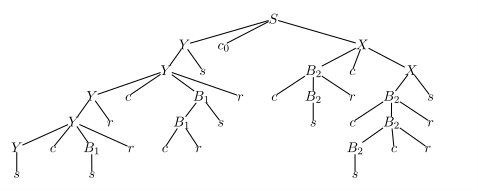
\includegraphics[scale=0.7]{sections/vpl_graph}
\caption{Schema des Syntaxbaumes}
\label{schema_tree}
\end{figure}
\end{lemma}

\begin{proof}
Sei Á ein passender Visibly Pushdown Automat, den wir als nichtdeterministsich annehmen (da äquivalent zur deterministischen Version \cite{vpl}) und $x=yc_0z$. Ohne Beschränkung der Allgemeinheit wird zusätzlch angenommen, dass der initiale Zustand $q_0$ nicht erneut erreicht wird.\\
Die Berechnung beginnt mit Transitionen zweiter und dritter Art, die $u_1$ einlesen, den Stack aber leer lassen. Dann beginnt der Automat $w_1$ einzulesen. Die erste Transition ist ein Push, bei der ein $Z_i \neq \bot$ auf den Stack gelegt wird. Danach folgen verschiedene Moves, die einen richtig balancierten String String einlesen, gefolgt von einer Pop-Transition, die genau $Z_i$ entfernt und so der richtig geschlossene String $w_1$ eingelesen wurde. Nun beginnt wieder das Einlesen von $u_2$ und so weiter bis $w_k$ vollständig eingelesen wurde. Es wird die Menge $Q_q$ von Zuständen definiert, die während des Lesens von y erreicht wurden.\\
An einem bestimmten Punkt, wenn der Stack leer und das Eingabesymbol in $\Sigma_c$ ist, ändert der Automat nichtdeterministisch sein Verhalten um $c_0z$ einzulesen. Es wird eine Menge $Q_p$ von Zuständen disjunkt von $Q_q \cup \{q_0\}$ definiert. Der Automat führt eine Push-Transition $\delta(r, c_0) \ni (r^\prime, Z_U)$ durch, wobei $Z_U$ ein Symbol auf dem Stack bezeichnet, dass nicht mehr durch eine Pop-Transition entfernt wird, also kann $c_0$ als unbeantworteter Call betrachtet werden. Dann wird z eingelesen, wobei zunächst ein richtig balancierter String $v_1$ eingelesen wird. Dann wird wieder nichtdeterministisch eine Push-Transition ausgeführt, in der wieder ein $Z_U$ auf den Stack gelegt wird. Schließlich endet die Berechnung irgendwann in einem akzeptierenden Zustand und einem Stack der Form $\bot Z_U^+$. Der String y steht für ein Wort (oder Präfix), dass mit einem leeren Stack endet.
\end{proof}


Bei der Konstruktion der Grammatik G wird für einen String x, der wie in \autoref{factorize} zerlegt wird, ein Syntaxbaum wie in \autoref{schema_tree}  konstruiert. Z.B. steht dabei das äußere linke s in \autoref{schema_tree} für den Substring $u_1$ im Lemma, $csr$ korrespondiert zu $w_1$ usw. 
In der Abbildung steht Y für ein Nichtterminal, dass einen String generiert, bei dem der Automat mit einem leeren Stack startet und endet.
Von Nichtterminalen $B_1, B_2$ werden richtig balancierte Strings abgeleitet. Nichtterminale X leiten Strings ab, sodass bei einem nichtleeren Stack $\bot Z_u^+$ kein Z gepoppt wird und am Ende einen String in $\bot Z_u^+$ enthalten ist. Die Nichtterminale der Grammatik (außer S) werden entweder als Paar $(q_i, q_j) , (p_i, p_j)$ oder als Tripel $(q_i, Z, q_j), (p_i, Z, q_j)$ mit $Z \in \Gamma$ beschrieben. Die Idee ist nun, dass Nichtterminale der Form $(t_i...t_j)$ einen Terminalstring u generieren, genau dann wenn es eine Berechnung des Automaten  von Zustand $t_i$ zu $t_j$ gibt, der den String einliest und den initialen Stack nicht poppt. Weiterhin steht $(q_i, q_j)$ für Nichtterminale, die den Stack unverändert lassen. Nichtterminale $(p_i, p_j)$ erhöhen, wenn überhaupt, die Anzahl an $Z_u$s und Nichtterminale $(q_i, Z, q_j)$ oder $(p_i, Z, p_j)$ bedeuten, dass die Berechnung mit Z oben auf dem Stack startet und endet, während ein richtig ausbalancierter String w gelesen wurde. Nun werden die Regeln für G aus den Transitionen in A abgeleitet: \\
Für die Ableitungen muss zwischen vielen Fällen abhängig von den Zerlegungen aus \ref{factorize}wie in \autoref{schema_tree} dargestellt, unterschieden werden. Diese Fälle sind in \autoref{table1} dargestellt.
Die so produzierte Grammatik ist nicht zwangsläufig reduziert, das heißt sie kann Regeln enthalten, deren linke Seite niemals in einer Ableitung des Startsymbols auftauchen. Diese nutzlosen Regeln können aber durch bekannte Algorithmen entfernt werden \cite{formallanguage}.
Damit eine Grammatik als Operatorpräzedenzgrammatik gilt, muss sie sich in Operatorform befinden und weiterhin eine konfliktfreie OPM haben. Durch die Konstruktion entstehen nur Regeln in Operatorform. Was die OPM angeht, so müssen für alle Regeln die relevanten Terminalmengen ($\mathcal{R}_G(A)$ oder $\mathcal{L}_G(A)$) gebildet werden. Hier wird das nur einmal exemplarisch gezeigt: \\
Für den Fall $Y \rightarrow YcBr$ mit der Regel $(q_0, q_n) \rightarrow (q_0, q_i)c(q_j, Z, q_m)r$ produziert $\mathcal{R}_G ((q_0,q_i))\subseteq \Sigma_i \cup \Sigma_r$ die Relationen $s \gtrdot c, \; r \gtrdot c$. Die Menge $\mathcal{L}_G ((q_j,Z q_m))\subseteq \Sigma_i \cup \Sigma_c$ produziert $c\lessdot c, \; c \lessdot s$ und aus $\mathcal{R}_G ((q_j,Z q_m))\subseteq \Sigma_i \cup \Sigma_r$ folgt $ s \gtrdot r, \; r \gtrdot r$. Die rechte Regelseite impliziert $c \doteq r$. Allein aus dieser Regel folgt eine konfliktfreie Matrix $M \subseteq M_T$, wobei $M_T$ die totale Matrix ist. Alle weiteren Regeln produzieren ähnliche Matrizen, die aber alle untereinander konfliktfrei sind. 
\begin{table}
\begin{center}

\begin{tabular}[c]{c | c | c | c }
	&	$\Sigma_c$ & $\Sigma_r$ & $\Sigma_i$ \\ \hline
$\Sigma_c$ & $\lessdot$ 	& $\doteq$	& $\lessdot$	\\ \hline
$\Sigma_r$ & $\gtrdot$	&$\gtrdot$		&$\gtrdot$		\\ \hline
$\Sigma_i$	&$\gtrdot$		&$\gtrdot$		&$\gtrdot$		\\
\end{tabular}
\caption{Totale Matrix $M_T$}
\label{tab2}
\end{center}
\end{table}
Die erwähnte totale Matrix hat immer die Form von \autoref{tab2}. Für alle Operatorpräzedenzgrammatiken mit einer solchen Matrix ist L(G) eine Visibly Pushdown Sprache \cite{op_vpl_property}.

\begin{table}
\scriptsize
\begin{tabular}{|l l l|}
\hline
Fall & Transitionen & Regeln in G \\
\hline \hline
$S \rightarrow Yc_0X$	& $\delta(q_i, c_0)	\ni (p_j, Z_U)$ & $S \rightarrow (q_0, q_i)c_0(p_i, p_f), \forall p_f \in Q_F$	\\
$S \rightarrow Y$	&	& $S \rightarrow (q_0, q_f), \forall q_f in Q_F$	\\
$S \rightarrow Yc_0$	& $\delta(q_i, c_0)	\ni (p_f, Z_U), q_f in Q_F$	& $S \rightarrow (q_0, q_f)c_0, \forall p_f \in Q_F$	\\
$S \rightarrow c_0Xs$	& $\delta(q_0, c_0)	\ni (p_j, Z_U)$	&$S \rightarrow c_0(q, p_j, p_f), \forall p_f \in Q_F$\\
$S \rightarrow c_0$	& $\delta(q_0, c_0)	\ni (p_f, Z_U), p_f \in Q_F$	&$S\rightarrow c_0$	\\
	\hline
$Y \rightarrow s$	& $\delta(q_0,s) \ni q_i$	& $(q_0, q_i) \rightarrow s$	\\
$Y \rightarrow r$	&$\delta(q_0,r, \bot) \ni q_i$	&	$(q_0, q_i) \rightarrow r$\\
$Y \rightarrow Ys$	&$\delta(q_i,s) \ni q_j$	& $(q_0, q_j) \rightarrow (q_0, q_i)s$	\\
$Y \rightarrow Yr$	&$\delta(q_i,r, \bot) \ni q_j$	&$(q_0, q_j) \rightarrow (q_0, q_i)r$	\\
$Y \rightarrow cBr$	&$\delta(q_0, c) \ni (q_t, Z), \; \delta(q_k,r, Z) \ni q_h$	& $(q_0, q_h) \rightarrow c(q_t, Z, q_k)r$	\\
$Y \rightarrow cr$	&$\delta(q_0, c) \ni (q_t, Z), \; \delta(q_t,r, Z) \ni q_h$	&$(q_0, q_h) \rightarrow cr$	\\
$Y \rightarrow YcBr$	&$\delta(q_i, c) \ni (q_j, Z), \; \delta(q_m,r, Z) \ni q_n$	& $(q_0, q_n) \rightarrow (q_0, q_i)c(q_j, Z, q_m)r$	\\
$Y \rightarrow Ycr$	&$\delta(q_i, c) \ni (q_j, Z), \; \delta(q_j,r, Z) \ni q_n$	& $(q_0, q_n) \rightarrow (q_0, q_i)cr$	\\
	\hline
$B_1 \rightarrow B_1cB_1r$	&$\delta(q_i, c) \ni (q_j, Z), \; \delta(q_m,r, Z) \ni q_n$	& $(q, q_n) \rightarrow (q, q_i)c(q_j, Z, q_m)r, \forall q \in Q_q$ \\
$B_1 \rightarrow B_1cr$	&$\delta(q_j, c) \ni (q_j, Z), \; \delta(q_j,r, Z) \ni q_n$	& $(q, q_n) \rightarrow(q, q_n)cr, \forall q \in Q_q$ \\
$B_1 \rightarrow cB_1r$	&$\delta(q_i, c) \ni (q_j, Z), \; \delta(q_m,r, Z) \ni q_n$	& $(q_i, q_n) \rightarrow c(q_j, Z, q_m)r$ \\
$B_1 \rightarrow cr$	&$\delta(q_i, c) \ni (q_j, Z), \; \delta(q_j,r, Z) \ni q_n$	& $(q_i, q_n) \rightarrow cr$ \\
$B_1 \rightarrow B_1cB_1r$	&$\delta(q_i, c) \ni (q_j, Z), \; \delta(q_m,r, Z) \ni q_n$	& $(q_i, W, q_n) \rightarrow (q, q_i)c(q_j, Z, q_m)r, \forall q \in Q_q, W \in \Gamma$ \\
$B_1 \rightarrow cB_1r$	&$\delta(q_i, c) \ni (q_j, Z), \; \delta(q_m,r, Z) \ni q_n$	& $(q, W, q_n) \rightarrow c(q_j, Z, q_m)r, \forall q \in Q_q, W \in \Gamma$ \\
$B_1 \rightarrow B_1cr$	&$\delta(q_i, c) \ni (q_j, Z), \; \delta(q_j,r, Z) \ni q_n$	& $(q, W, q_n) \rightarrow (q, q_i)cr, \forall q \in Q_q, W \in \Gamma$ \\
$B_1 \rightarrow B_1s$	&$\delta(q_h, s) \ni q_m$ & $(q, W, q_m) \rightarrow (q, q_h)s, \forall q \in Q_q, W \in \Gamma$ \\
$B_1 \rightarrow s$	&$\delta(q_j, s) \ni q_m$ & $(q_j, W, q_m) \rightarrow s, \forall W \in \Gamma$ \\
\hline
$B_2 \rightarrow B_2cB_2r$	&$\delta(q_i, c) \ni (q_j, Z), \; \delta(q_m,r, Z) \ni q_n$	& $(p, q_n) \rightarrow (p, q_i)c(q_j, Z, q_m)r, \forall p \in Q_p$ \\
$B_2 \rightarrow B_2cr$	&$\delta(q_j, c) \ni (q_j, Z), \; \delta(q_j,r, Z) \ni q_n$	& $(p, q_n) \rightarrow(p, q_n)cr, \forall p \in Q_p$ \\
$B_2 \rightarrow cB_2r$	&$\delta(q_i, c) \ni (q_j, Z), \; \delta(q_m,r, Z) \ni q_n$	& $(q_i, q_n) \rightarrow c(q_j, Z, q_m)r$ \\
$B_2 \rightarrow cr$	&$\delta(q_i, c) \ni (q_j, Z), \; \delta(q_j,r, Z) \ni q_n$	& $(q_i, q_n) \rightarrow cr$ \\
$B_2 \rightarrow B_2cB_2r$	&$\delta(q_i, c) \ni (q_j, Z), \; \delta(q_m,r, Z) \ni q_n$	& $(q_i, W, q_n) \rightarrow (p, q_i)c(q_j, Z, q_m)r, \forall p \in Q_p, W \in \Gamma$ \\
$B_2 \rightarrow cB_2r$	&$\delta(q_i, c) \ni (q_j, Z), \; \delta(q_m,r, Z) \ni q_n$	& $(p, W, q_n) \rightarrow c(q_j, Z, q_m)r, \forall p \in Q_p, W \in \Gamma$ \\
$B_2 \rightarrow B_2cr$	&$\delta(q_i, c) \ni (q_j, Z), \; \delta(q_j,r, Z) \ni q_n$	& $(p, W, q_n) \rightarrow (p, q_i)cr, \forall p \in Q_p, W \in \Gamma$ \\
$B_2 \rightarrow B_2s$	&$\delta(q_h, s) \ni q_m$ & $(q, W, q_m) \rightarrow (p, q_h)s, \forall p \in Q_p, W \in \Gamma$ \\
$B_2 \rightarrow s$	&$\delta(q_j, s) \ni q_m$ & $(q_j, W, q_m) \rightarrow s, \forall W \in \Gamma$ \\
\hline
$X \rightarrow cX$	&$\delta(p_i, c) \ni (p_j, Z_U)$ & $(p_i, p_f) \rightarrow c(p_j, p_f), \forall p_f \in Q_F$ \\
$X \rightarrow c$	&$\delta(p_i, c) \ni (p_f, Z_U), p_f \in Q_F$ & $(p_i, p_f) \rightarrow c$ \\
$X \rightarrow BcX$	&$\delta(p_j, c) \ni (p_h, Z_U)$ & $(p, p_f) \rightarrow (p, p_j)c(p_h, p_f), \forall p_f \in Q_F, p \in Q_p$ \\
$X \rightarrow Bc$	&$\delta(p_j, c) \ni (p_f, Z_U), p_f \in Q_F$ & $(p, p_f) \rightarrow (p, p_j)c$ \\
$X \rightarrow BcBr$	&$\delta(p_i, c) \ni (p_j, Z), \delta(p_m, r, Z) \ni p_n$ & $(p, p_f) \rightarrow (p, p_i)c(p_j, Z, p_m)r, \forall p_f \in Q_F, p \in Q_p$ \\
$X \rightarrow cBr$	&$\delta(p_i, c) \ni (p_j, Z), \delta(p_m, r, Z) \ni p_n$ & $(p_i, p_f) \rightarrow c(p_j, Z, p_n)r, \forall p_f \in Q_F$ \\
$X \rightarrow cr$	&$\delta(p_i, c) \ni (p_j, Z), \delta(p_j, r, Z) \ni p_n$ & $(p_i, p_f) \rightarrow c(p_j, Z, p_n)r, \forall p_f \in Q_F$ \\
$X \rightarrow Bs$	&$\delta(p_j, s) \ni p_f, p_f \in Q_F$ & $(p, p_f) \rightarrow (p, p_j)s, \forall p \in Q_p$ \\
$X \rightarrow s$	&$\delta(p_j, s) \ni p_f, p_f \in Q_F$ & $(p, p_f) \rightarrow s$ \\ 
\hline
\end{tabular}

\caption{Übersicht der Regelgeneration}
\label{table1}
\end{table}
\end{proof}